\section{Formeln}
\subsection{Weg-Zeit Berechnung}
Für die im folgenden Abschnitt verwendeten Gleichungen gilt:
\begin{conditions}
a     &  Bremsverzoegerung [$m/s^{2}$] \\
v     &  Geschwindigkeit [$m/s$] \\
s     &  Strecke [$m$] \\
t     &  Zeit [$s$]
\end{conditions}
\noindent Bei einer konstanten Beschleunigung gilt:
\begin{equation}
a(t) = a
\end{equation}
Für die Bestimmung der Geschwindigkeit in Abhängigkeit der Zeit, muss die Beschleunigung $a(t)$ nach der Zeit $t$ integriert werden.\footnote{\citet[S. 20]{richard2011technische}}
\begin{equation}
v(t) = \int a(t) \,dt
\end{equation}
Daraus ergibt sich folgende Gleichung für die Geschwindigkeit in Abhängigkeit der Zeit. Die bei der Integration entstehende Integrationskonstante $v_{0}$ gibt dabei die Startgeschwindigkeit an.
\begin{equation}
v(t) = a \cdot t + v_{0}
\end{equation}
Für die Bestimmung der benötigten Zeit muss die Geschwindigkeit erneut integriert werden.\footnote{ebd. (S. 20)} Die dabei entstehende Integrationskonstante $s_{0}$ gibt dabei die bereits zurückgelegte Strecke an.
\begin{equation}
s(t) = \int v(t) \,dt
\end{equation}
\begin{equation}
s(t) =\frac{1}{2} \cdot a \cdot t^{2} + v_{0}  \cdot t + s_{0}
\end{equation}
Bei der Verwendung dieser Gleichung werden die Integrationskonstanten $v_{0}$ und $s_{0}$ gleich $0$ gesetzt, damit die Gleichungen allgemein gültig sind. Für die Berechnung des Beschleuniguns- und Abbremsverhalten der Fahrzeuge ist es notwendig zu wissen, welche Strecke ein Fahrzeug zurücklegen muss, um von einer Startgeschwindigkeit $v_{0}$ auf eine Zielgeschwindigkeit $v_{1}$ zu beschleunigen bzw. abzubremsen. Dafür wird die Gleichung für die Geschwindigkeit $v(t)$ nach $t$ umgestellt und und in die Gleichung $s(t)$ eingesetzt. Daraus ergibt sich folgende Gleichung für die Strecke in Abhängigkeit von der Geschwindigkeit:
\begin{equation}
t(v) = \frac{v}{a}
\end{equation}
\begin{equation}
s(v) =\frac{1}{2} \cdot \frac{v^{2}}{a}
\end{equation}
Durch die Festlegung von $v_{0} = 0$ wird so die benötigte Strecke ermittelt, welche ein Fahrzeug bei einer gegebenen Bremsverzögerung $a$ benötigt, um von 0 $m/s$ auf eine gegebenen Zielgeschwindigkeit $v_{1}$ zu beschleunigen. Bei der Berechnung des Beschleuniguns- und Abbremsverhalten wird es aber auch zu Situationen kommen, bei denen ein Fahrzeug eine Startgeschwindigkeit hat, für die gilt $v_{0} \neq 0$. Um eine allgemein gültige Gleichung aufzustellen, wird für die Ermittlung der benötigten Strecke bei einer gegebenen Start- und Zielgeschwindigkeit die Strecke berechnet, die das Fahrzeug benötigt um von 0 $m/s$ auf $v_{1}$ zu beschleunigen und von 0 $m/s$ auf $v_{0}$. Für die gesuchte Strecke gilt dann: 
\begin{equation}
s(v_{0}, v_{1}) = s(v_{1}) - s(v_{0}) 
\end{equation}
\begin{equation}
\label{eq:s_v_ges}
s(v_{0}, v_{1}) =\frac{1}{2} \cdot \frac{v_{1}^{2} - v_{0}^{2}}{a}
\end{equation}
In dem Programm übernimmt diese Berechnung die Funktion \textit{getBrakeDistance()}. Damit keine negativen Rückgabewerte entstehen, wird im Falle einer Bremsung ($v_{1} \textless v_{0}$) das Ergebnis mit $-1$ multipliziert. Beispiel eines Querverweis \eqref{eq:s_v_ges}.
\begin{lstlisting}
function getBrakeDistance (float $v_0, float $v_1, float $verzoegerung) {
	if ($v_0 > $v_1) {
		return $bremsweg = 0.5 * ((pow($v_0/3.6,2)-pow($v_1/3.6, 2))/($verzoegerung));
	} else if ($v_0 < $v_1) {
		return $bremsweg = -0.5 * ((pow($v_0/3.6,2)-pow($v_1/3.6, 2))/($verzoegerung));
	} else {
		return 0;
	}
}
\end{lstlisting}
Neben der Berechnung der Strecke ist auch die benötigte Zeit essenziell. Dafür wird mittels $t(v)$ die Zeit berechnet, die das Fahrzeug benötigt, um von $v_{0}$ auf $v_{1}$ zu beschleunigen bzw. abzubremsen und aus der Differenz die benötigte Zeit berechnet.
\begin{equation}
t(v_{0}, v_{1}) = \frac{v_{1} - v_{0}}{a}
\end{equation}
In dem Programm übernimmt diese Berechnung die Funktion \textit{getBrakeTime()}. Damit keine negativen Rückgabewerte entstehen, wird im Falle einer Bremsung ($v_{1} \textless v_{0}$) das Ergebnis mit $-1$ multipliziert.
\begin{lstlisting}
function getBrakeTime (float $v_0, float $v_1, float $verzoegerung) {
	if ($v_0 < $v_1) {
		return (($v_1/3.6)/$verzoegerung) - (($v_0/3.6)/$verzoegerung);
	} else if ($v_0 > $v_1) {
		return (($v_0/3.6)/$verzoegerung) - (($v_1/3.6)/$verzoegerung);
	} else {
		return 0;
	}
}
\end{lstlisting}
\subsection{Teil 2}
\begin{table}[]
\begin{center}
\renewcommand{\arraystretch}{1.2}
\begin{tabular}[h]{c| C{3cm} |c}
Infrastrukturabschnitts-ID & Länge & zulässige Höchstgeschwindigkeit \\ \hline
1000                   &   300 $m$    & 120 $km/h$                        \\ \hline
1001                  &    400 $m$   & 120 $km/h$                        \\ \hline
1002                   &   300 $m$    &        120 $km/h$                         \\ \hline
1003                   &    400 $m$   &         90 $km/h$                        \\ \hline
1004                   &    300 $m$   &            60 $km/h$                     \\ \hline
1005                   &   200 $m$    &           60 $km/h$                      \\ \hline
1006                   &  400 $m$     &      90 $km/h$                           \\ \hline
1007                   &  500 $m$     &      120 $km/h$                           \\ \hline
1008                   &   300 $m$    &      120 $km/h$                           \\ \hline
1009                   &   400 $m$    &      100 $km/h$                           \\ \hline
1010                   &   300 $m$    &      60 $km/h$                           \\ \hline
1011                   &   300 $m$    &         40 $km/h$                        \\ 
\end{tabular}
\renewcommand{\arraystretch}{1}
\caption{Beispiel Infrastrukturabschnitte}
\end{center}
\end{table}
Lorem ipsum dolor sit amet, consetetur sadipscing elitr, sed diam nonumy eirmod tempor invidunt ut labore et dolore magna aliquyam erat, sed diam voluptua. At vero eos et accusam et justo duo dolores et ea rebum. Stet clita kasd gubergren, no sea takimata sanctus est Lorem ipsum dolor sit amet. Lorem ipsum dolor sit amet, consetetur sadipscing elitr, sed diam nonumy eirmod tempor invidunt ut labore et dolore magna aliquyam erat, sed diam voluptua. At vero eos et accusam et justo duo dolores et ea rebum. Stet clita kasd gubergren, no sea takimata sanctus est Lorem ipsum dolor sit amet.
\begin{table}[]
\begin{center}
\renewcommand{\arraystretch}{1.2}
\begin{tabular}[h]{r L{3cm}}

relative Startposition                   &   10 $m$                         \\ 
relative Zielposition                  &    290 $m$                         \\ 
aktueller Infrastrukturabschnitt                   &   1001                         \\ 
Ziel-Infrastrukturabschnitt                  &    1010                         \\ 
Startgeschwindigkeit                   &   0 $km/h$                          \\ 
Zielgeschwindigkeit                   &    0 $km/h$                        \\ 
Zuglänge                   &    50 $m$                        \\ 
Bremsverzögerung                   &    0,8 $m/s^{2}$                        \\ 
Fahrplan vorhanden                   &    ja                        \\ 
Zeit bis zur nächsten Betriebsstelle                   &    210 $s$                        \\ 

\end{tabular}
\renewcommand{\arraystretch}{1}
\caption{Beispiel Zugdaten}
\end{center}
\end{table}
Lorem ipsum dolor sit amet, consetetur sadipscing elitr, sed diam nonumy eirmod tempor invidunt ut labore et dolore magna aliquyam erat, sed diam voluptua. At vero eos et accusam et justo duo dolores et ea rebum. Stet clita kasd gubergren, no sea takimata sanctus est Lorem ipsum dolor sit amet. Lorem ipsum dolor sit amet, consetetur sadipscing elitr, sed diam nonumy eirmod tempor invidunt ut labore et dolore magna aliquyam erat, sed diam voluptua. At vero eos et accusam et justo duo dolores et ea rebum. Stet clita kasd gubergren, no sea takimata sanctus est Lorem ipsum dolor sit amet. Lorem ipsum dolor sit amet, consetetur sadipscing elitr, sed diam nonumy eirmod tempor invidunt ut labore et dolore magna aliquyam erat, sed diam voluptua. At vero eos et accusam et justo duo dolores et ea rebum. Stet clita kasd gubergren, no sea takimata sanctus est Lorem ipsum dolor sit amet. Lorem ipsum dolor sit amet, consetetur sadipscing elitr, sed diam nonumy eirmod tempor invidunt ut labore et dolore magna aliquyam erat, sed diam voluptua. At vero eos et accusam et justo duo dolores et ea rebum. Stet clita kasd gubergren, no sea takimata sanctus est Lorem ipsum dolor sit amet. In der nächsten Darstellung sind die beispielhaften Infrastruktabschnitte bildlich dargestellt. Auf der x-Achse ist die Strecke in Metern angegeben und auf der y-Achse die zulässige Höchstgeschwindigkeit.
\begin{figure}[H]
  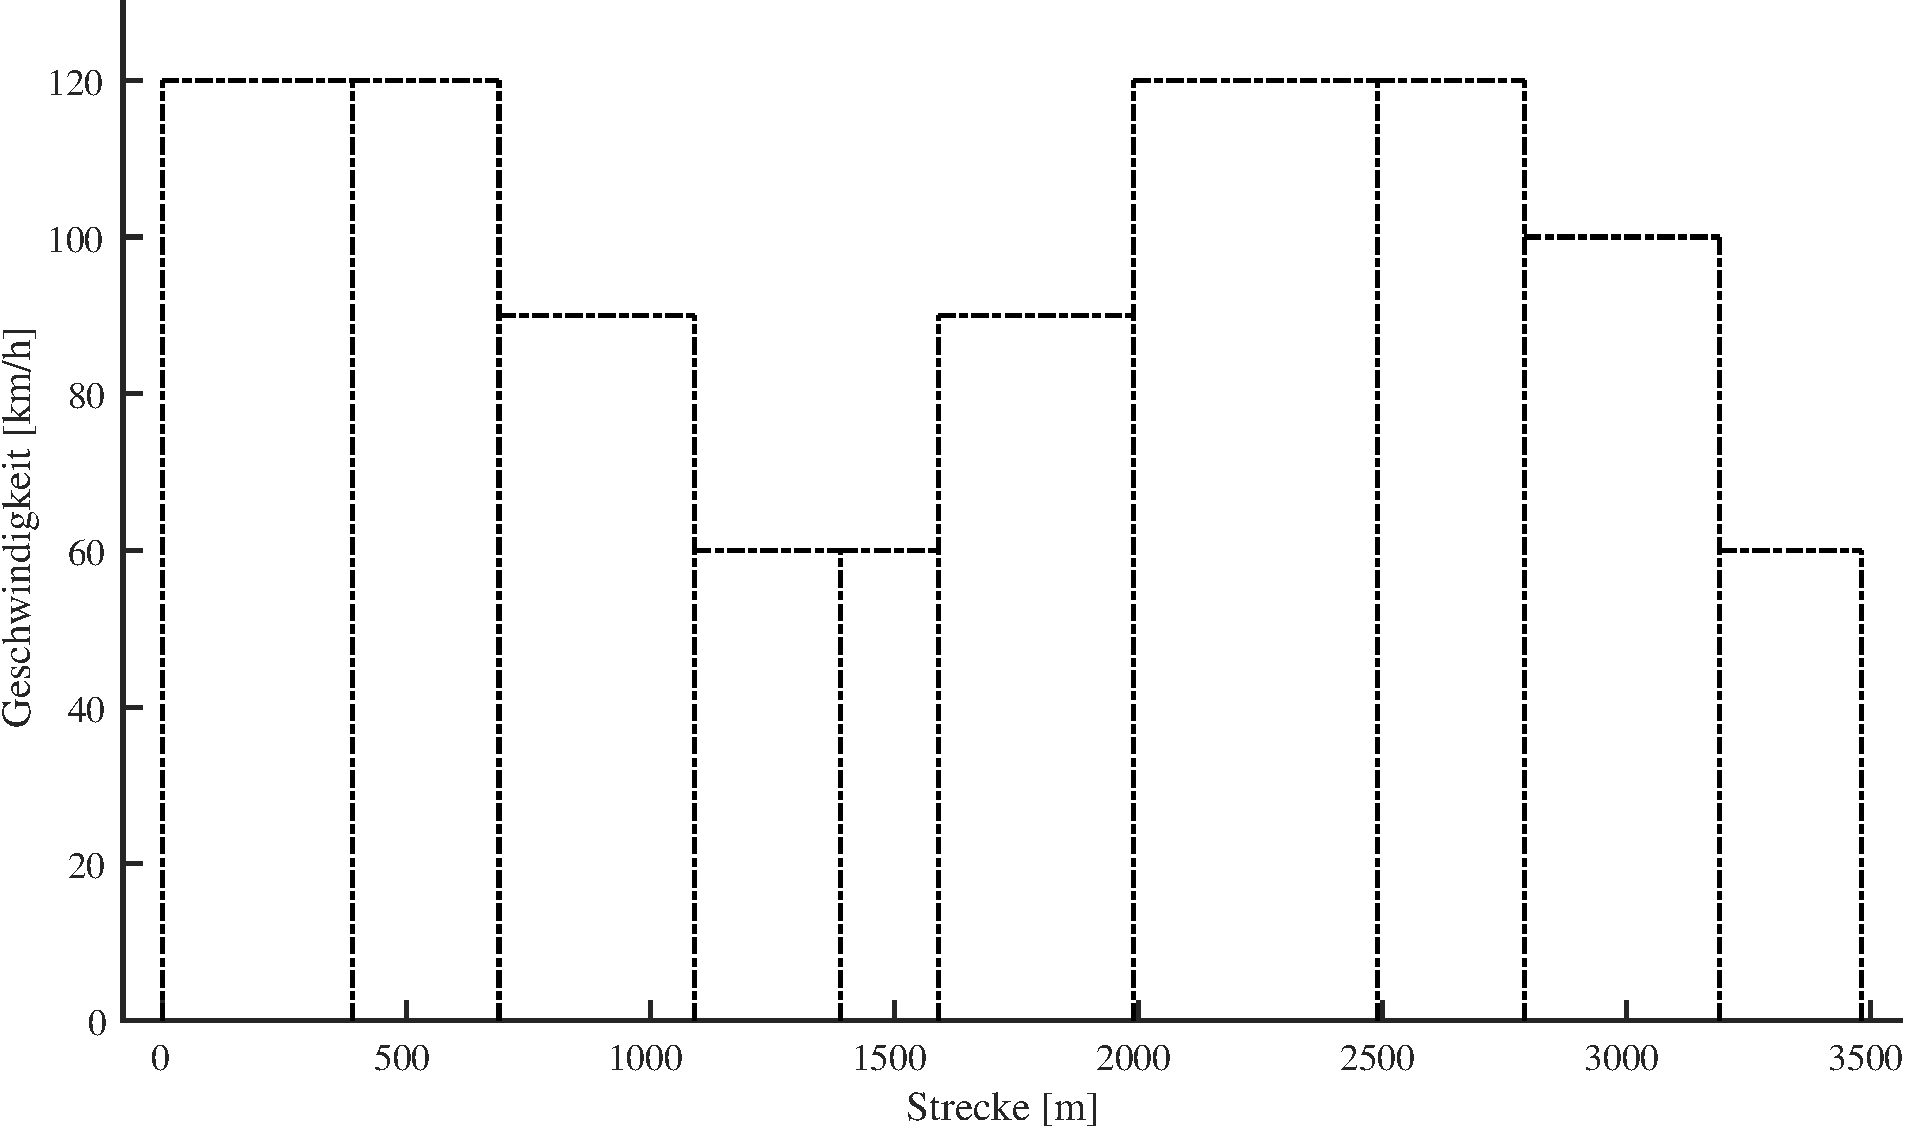
\includegraphics[width=\linewidth]{../matlab/it_0_1.pdf}
  \caption{Darstellung der Geschwindigkeit des Fahrzeugs über die Strecke}
\end{figure}
Lorem ipsum dolor sit amet, consetetur sadipscing elitr, sed diam nonumy eirmod tempor invidunt ut labore et dolore magna aliquyam erat, sed diam voluptua. At vero eos et accusam et justo duo dolores et ea rebum. Stet clita kasd gubergren, no sea takimata sanctus est Lorem ipsum dolor sit amet. Lorem ipsum dolor sit amet, consetetur sadipscing elitr, sed diam nonumy eirmod tempor invidunt ut labore et dolore magna aliquyam erat, sed diam voluptua. At vero eos et accusam et justo duo dolores et ea rebum. Stet clita kasd gubergren, no sea takimata sanctus est Lorem ipsum dolor sit amet.
\begin{figure}[H]
  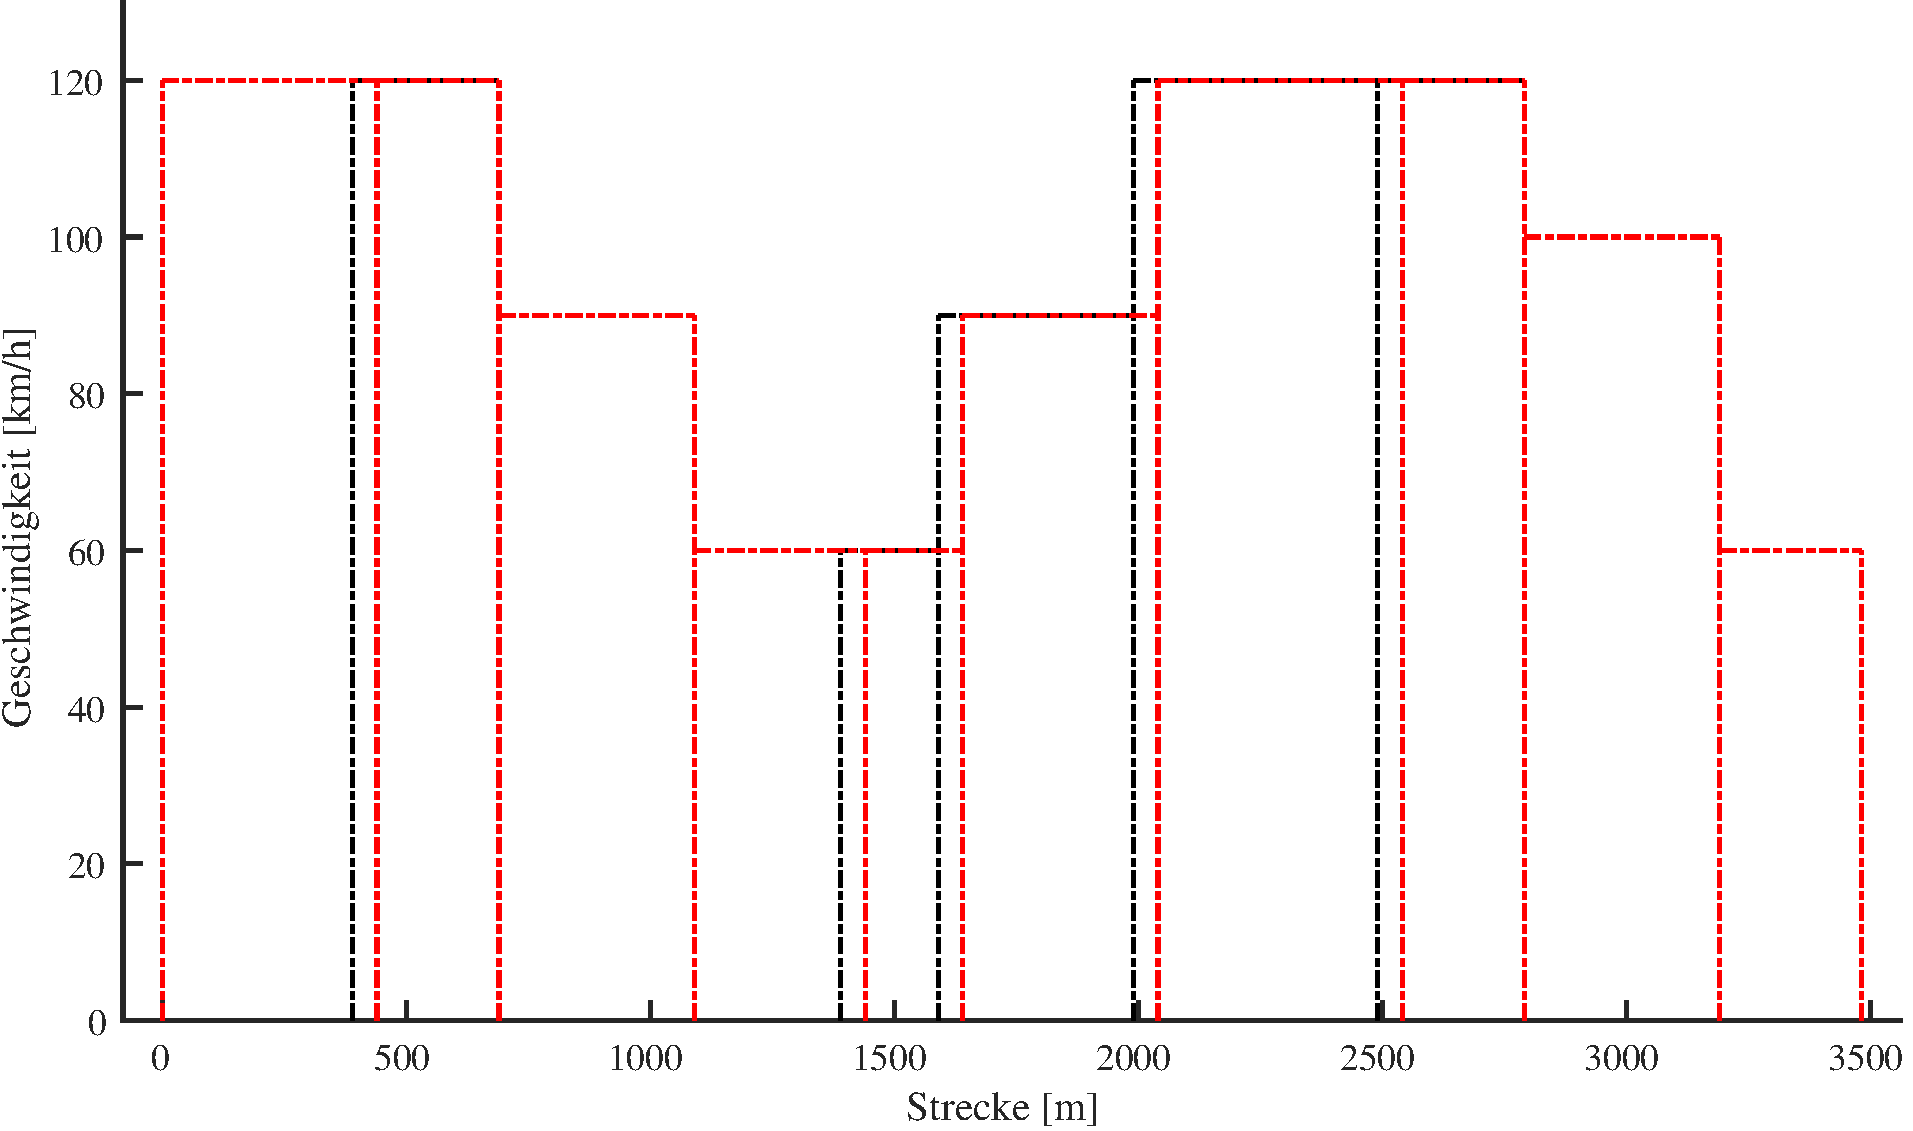
\includegraphics[width=\linewidth]{../matlab/it_0_2.pdf}
  \caption{Darstellung der Geschwindigkeit des Fahrzeugs über die Strecke}
\end{figure}
Lorem ipsum dolor sit amet, consetetur sadipscing elitr, sed diam nonumy eirmod tempor invidunt ut labore et dolore magna aliquyam erat, sed diam voluptua. At vero eos et accusam et justo duo dolores et ea rebum. Stet clita kasd gubergren, no sea takimata sanctus est Lorem ipsum dolor sit amet. Lorem ipsum dolor sit amet, consetetur sadipscing elitr, sed diam nonumy eirmod tempor invidunt ut labore et dolore magna aliquyam erat, sed diam voluptua. At vero eos et accusam et justo duo dolores et ea rebum. Stet clita kasd gubergren, no sea takimata sanctus est Lorem ipsum dolor sit amet.
\begin{figure}[H]
  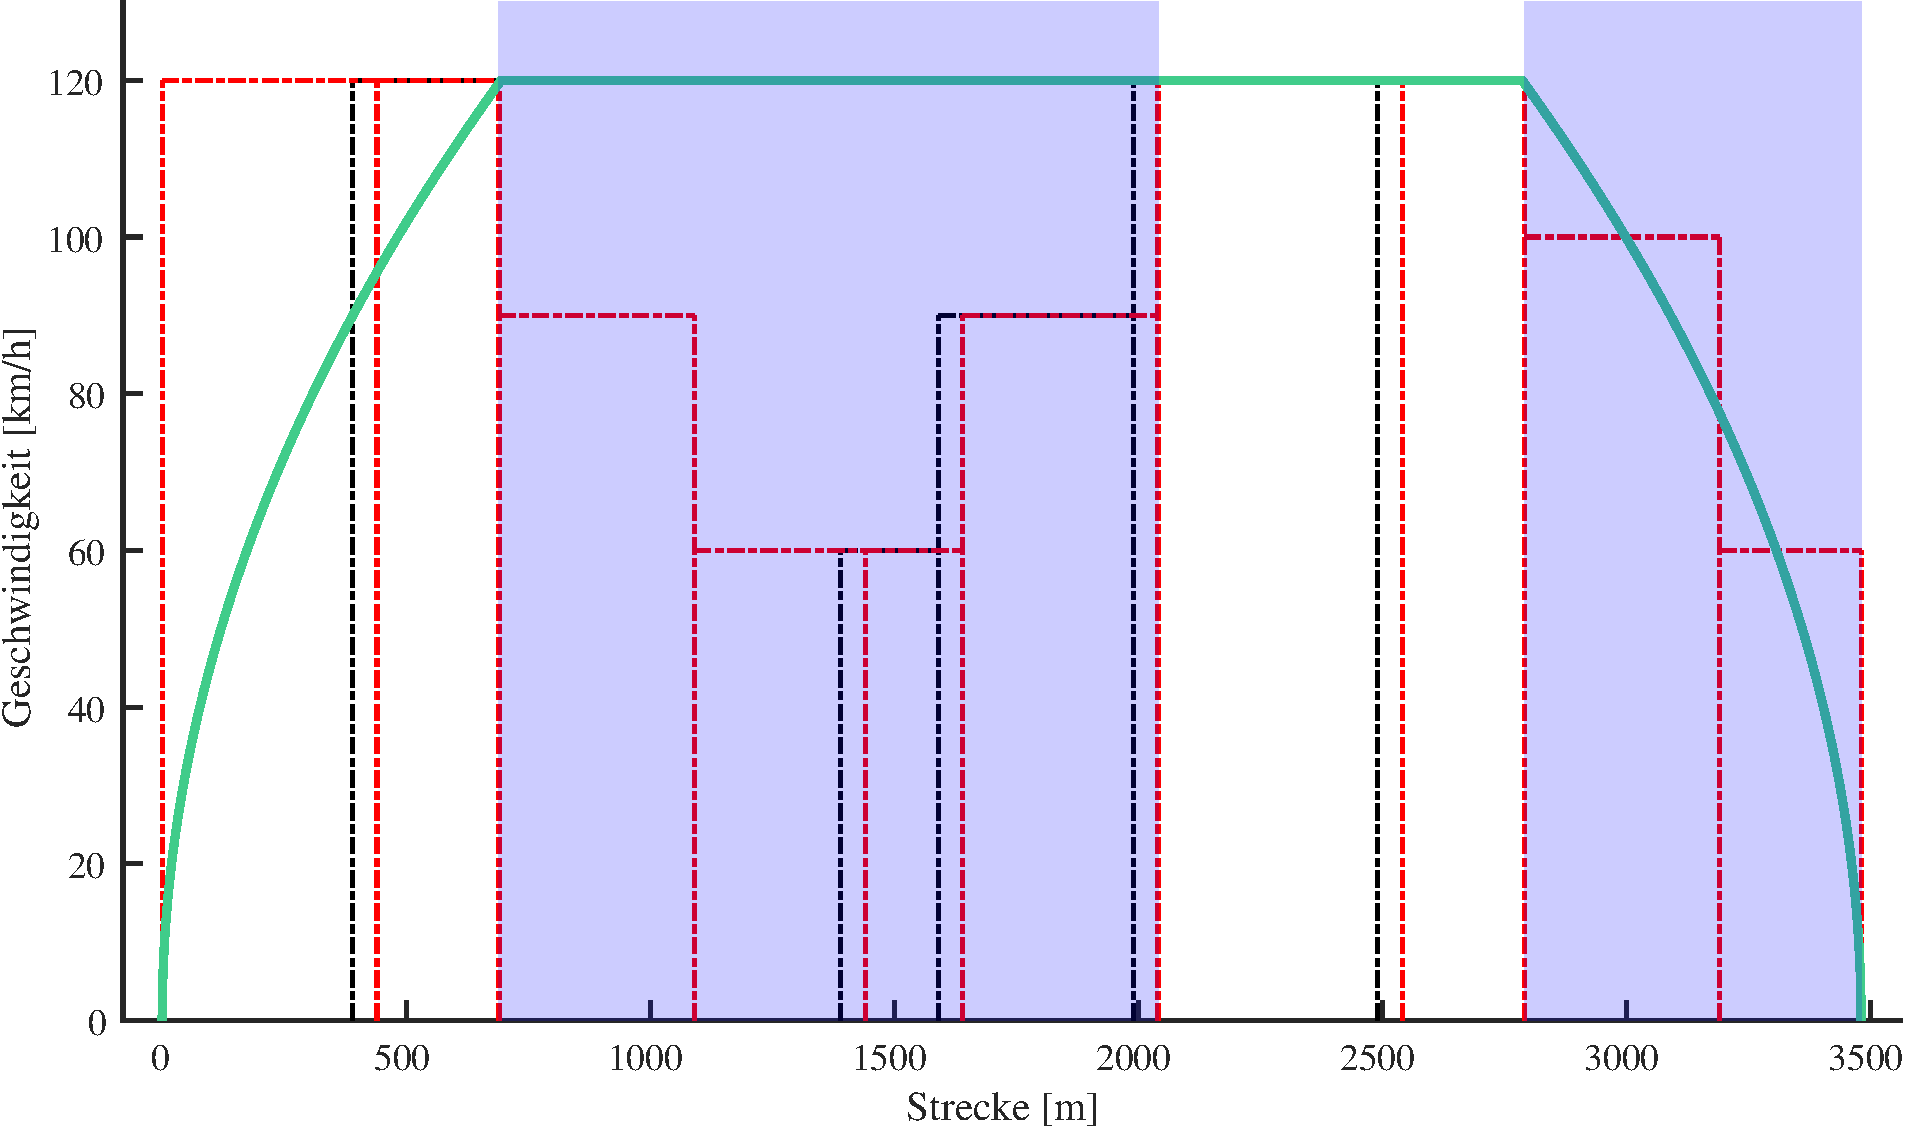
\includegraphics[width=\linewidth]{../matlab/it_1.pdf}
  \caption{Darstellung der Geschwindigkeit des Fahrzeugs über die Strecke}
\end{figure}
Lorem ipsum dolor sit amet, consetetur sadipscing elitr, sed diam nonumy eirmod tempor invidunt ut labore et dolore magna aliquyam erat, sed diam voluptua. At vero eos et accusam et justo duo dolores et ea rebum. Stet clita kasd gubergren, no sea takimata sanctus est Lorem ipsum dolor sit amet. Lorem ipsum dolor sit amet, consetetur sadipscing elitr, sed diam nonumy eirmod tempor invidunt ut labore et dolore magna aliquyam erat, sed diam voluptua. At vero eos et accusam et justo duo dolores et ea rebum. Stet clita kasd gubergren, no sea takimata sanctus est Lorem ipsum dolor sit amet.
\begin{figure}[H]
  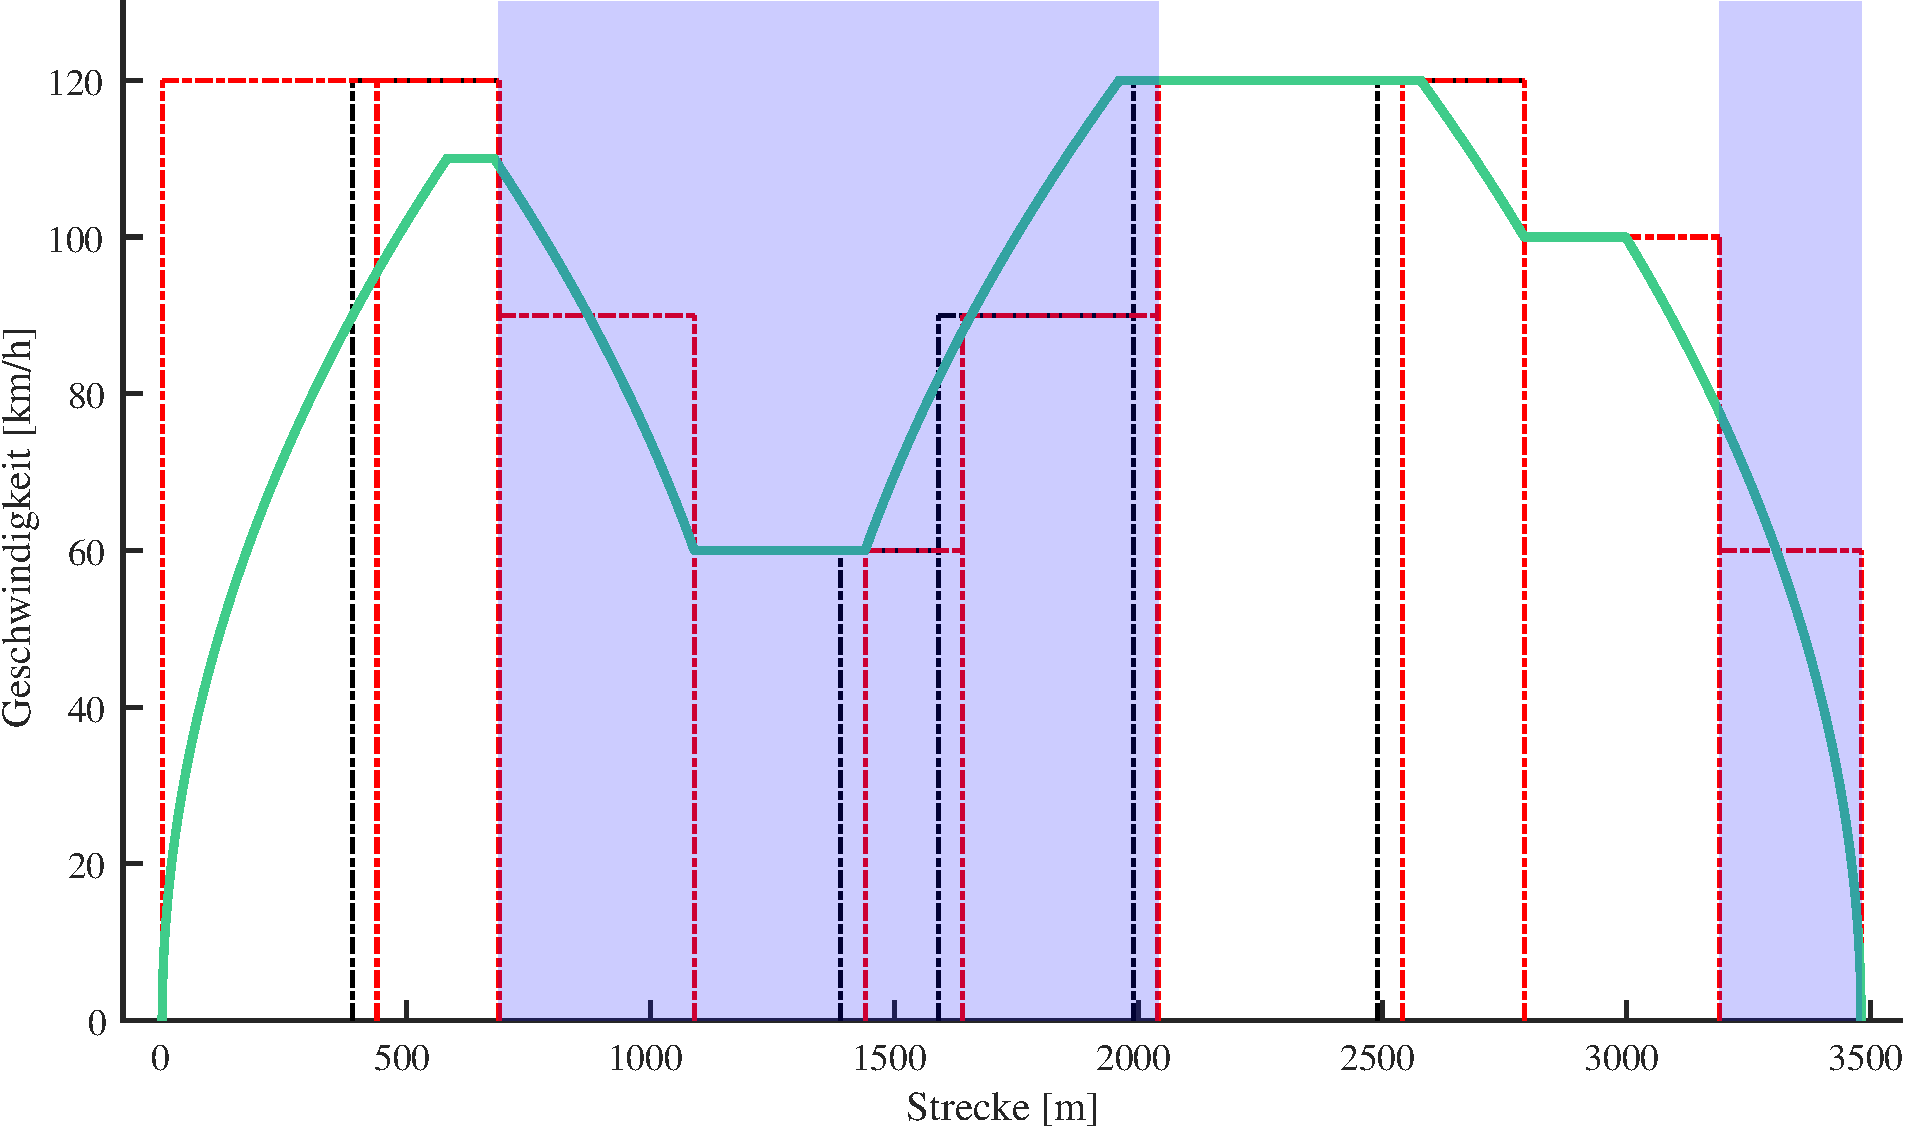
\includegraphics[width=\linewidth]{../matlab/it_2.pdf}
  \caption{Darstellung der Geschwindigkeit des Fahrzeugs über die Strecke}
\end{figure}
Lorem ipsum dolor sit amet, consetetur sadipscing elitr, sed diam nonumy eirmod tempor invidunt ut labore et dolore magna aliquyam erat, sed diam voluptua. At vero eos et accusam et justo duo dolores et ea rebum. Stet clita kasd gubergren, no sea takimata sanctus est Lorem ipsum dolor sit amet. Lorem ipsum dolor sit amet, consetetur sadipscing elitr, sed diam nonumy eirmod tempor invidunt ut labore et dolore magna aliquyam erat, sed diam voluptua. At vero eos et accusam et justo duo dolores et ea rebum. Stet clita kasd gubergren, no sea takimata sanctus est Lorem ipsum dolor sit amet.
\begin{figure}[H]
  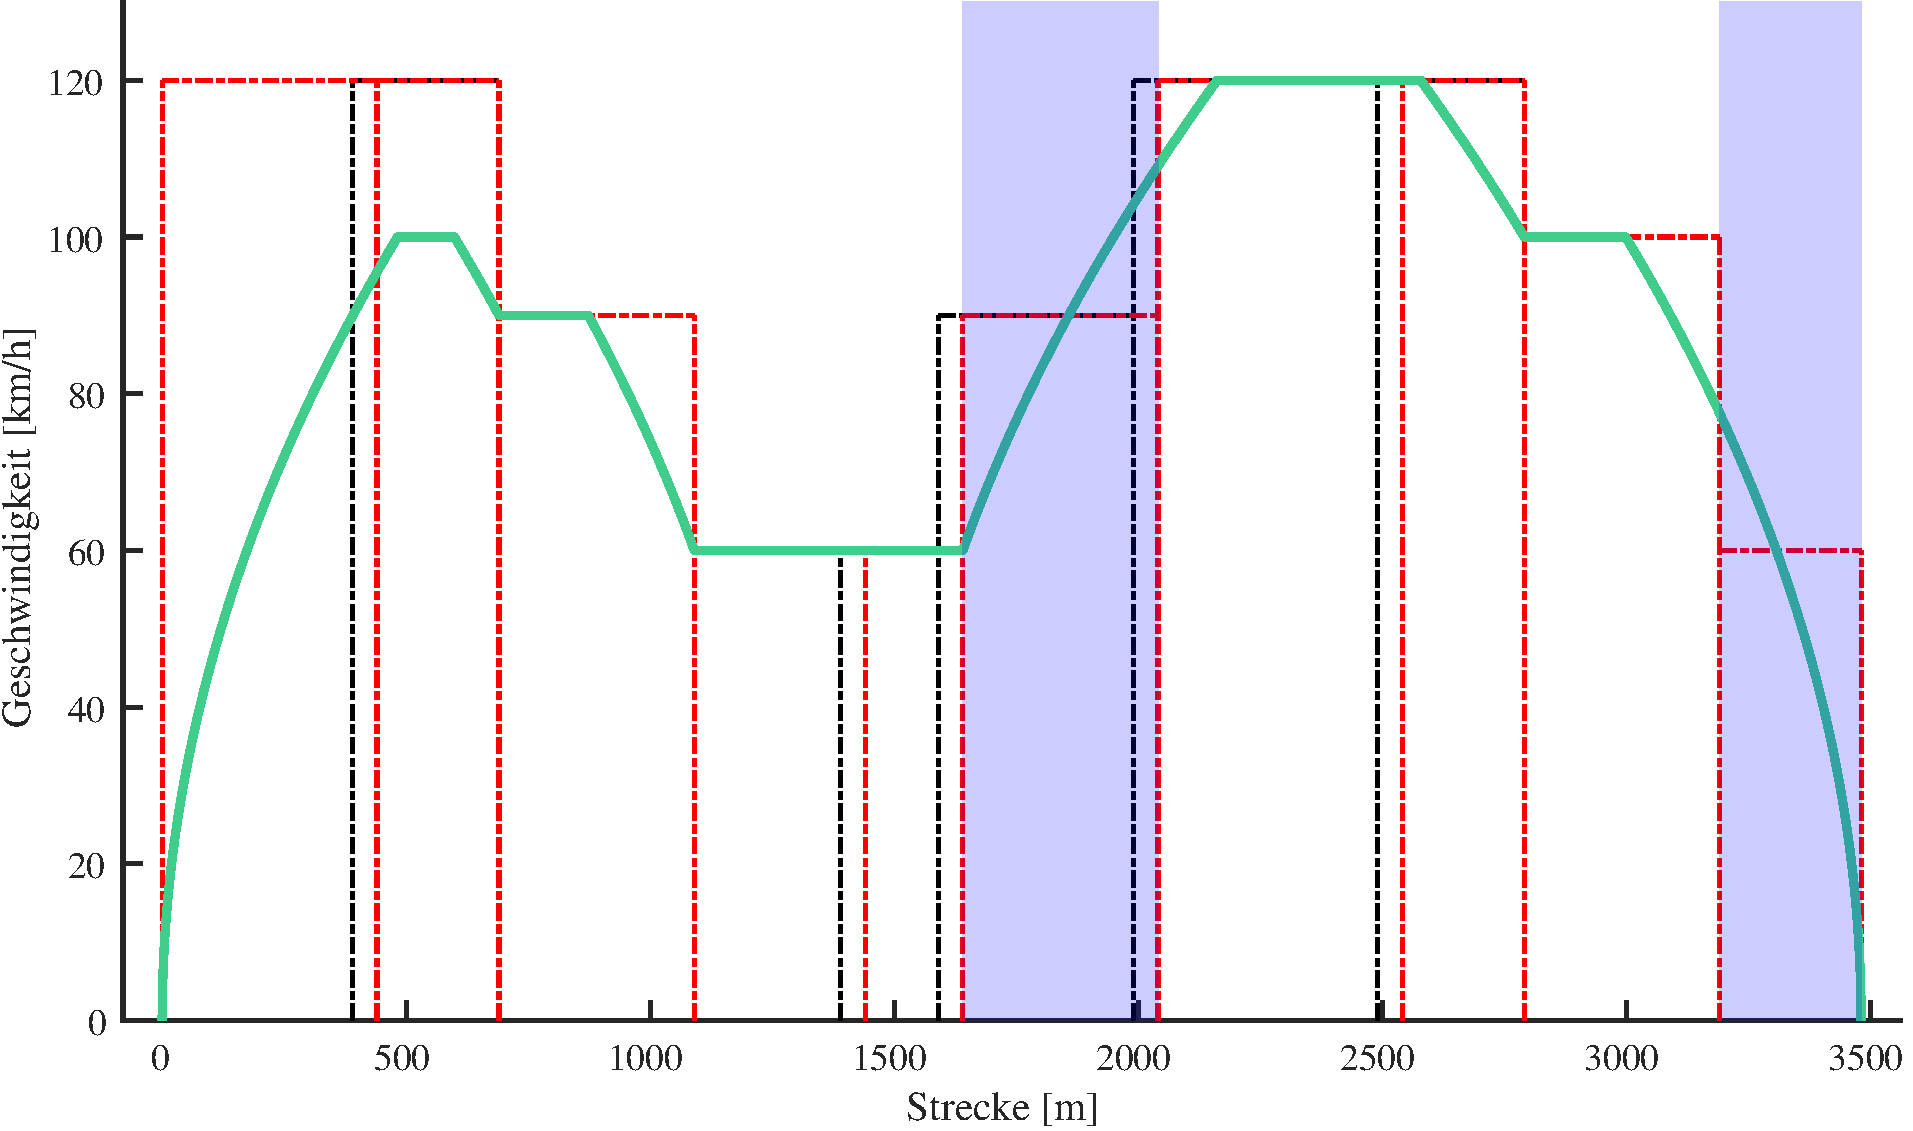
\includegraphics[width=\linewidth]{../matlab/it_3.pdf}
  \caption{Darstellung der Geschwindigkeit des Fahrzeugs über die Strecke}
\end{figure}
Lorem ipsum dolor sit amet, consetetur sadipscing elitr, sed diam nonumy eirmod tempor invidunt ut labore et dolore magna aliquyam erat, sed diam voluptua. At vero eos et accusam et justo duo dolores et ea rebum. Stet clita kasd gubergren, no sea takimata sanctus est Lorem ipsum dolor sit amet. Lorem ipsum dolor sit amet, consetetur sadipscing elitr, sed diam nonumy eirmod tempor invidunt ut labore et dolore magna aliquyam erat, sed diam voluptua. At vero eos et accusam et justo duo dolores et ea rebum. Stet clita kasd gubergren, no sea takimata sanctus est Lorem ipsum dolor sit amet.
\begin{figure}[H]
  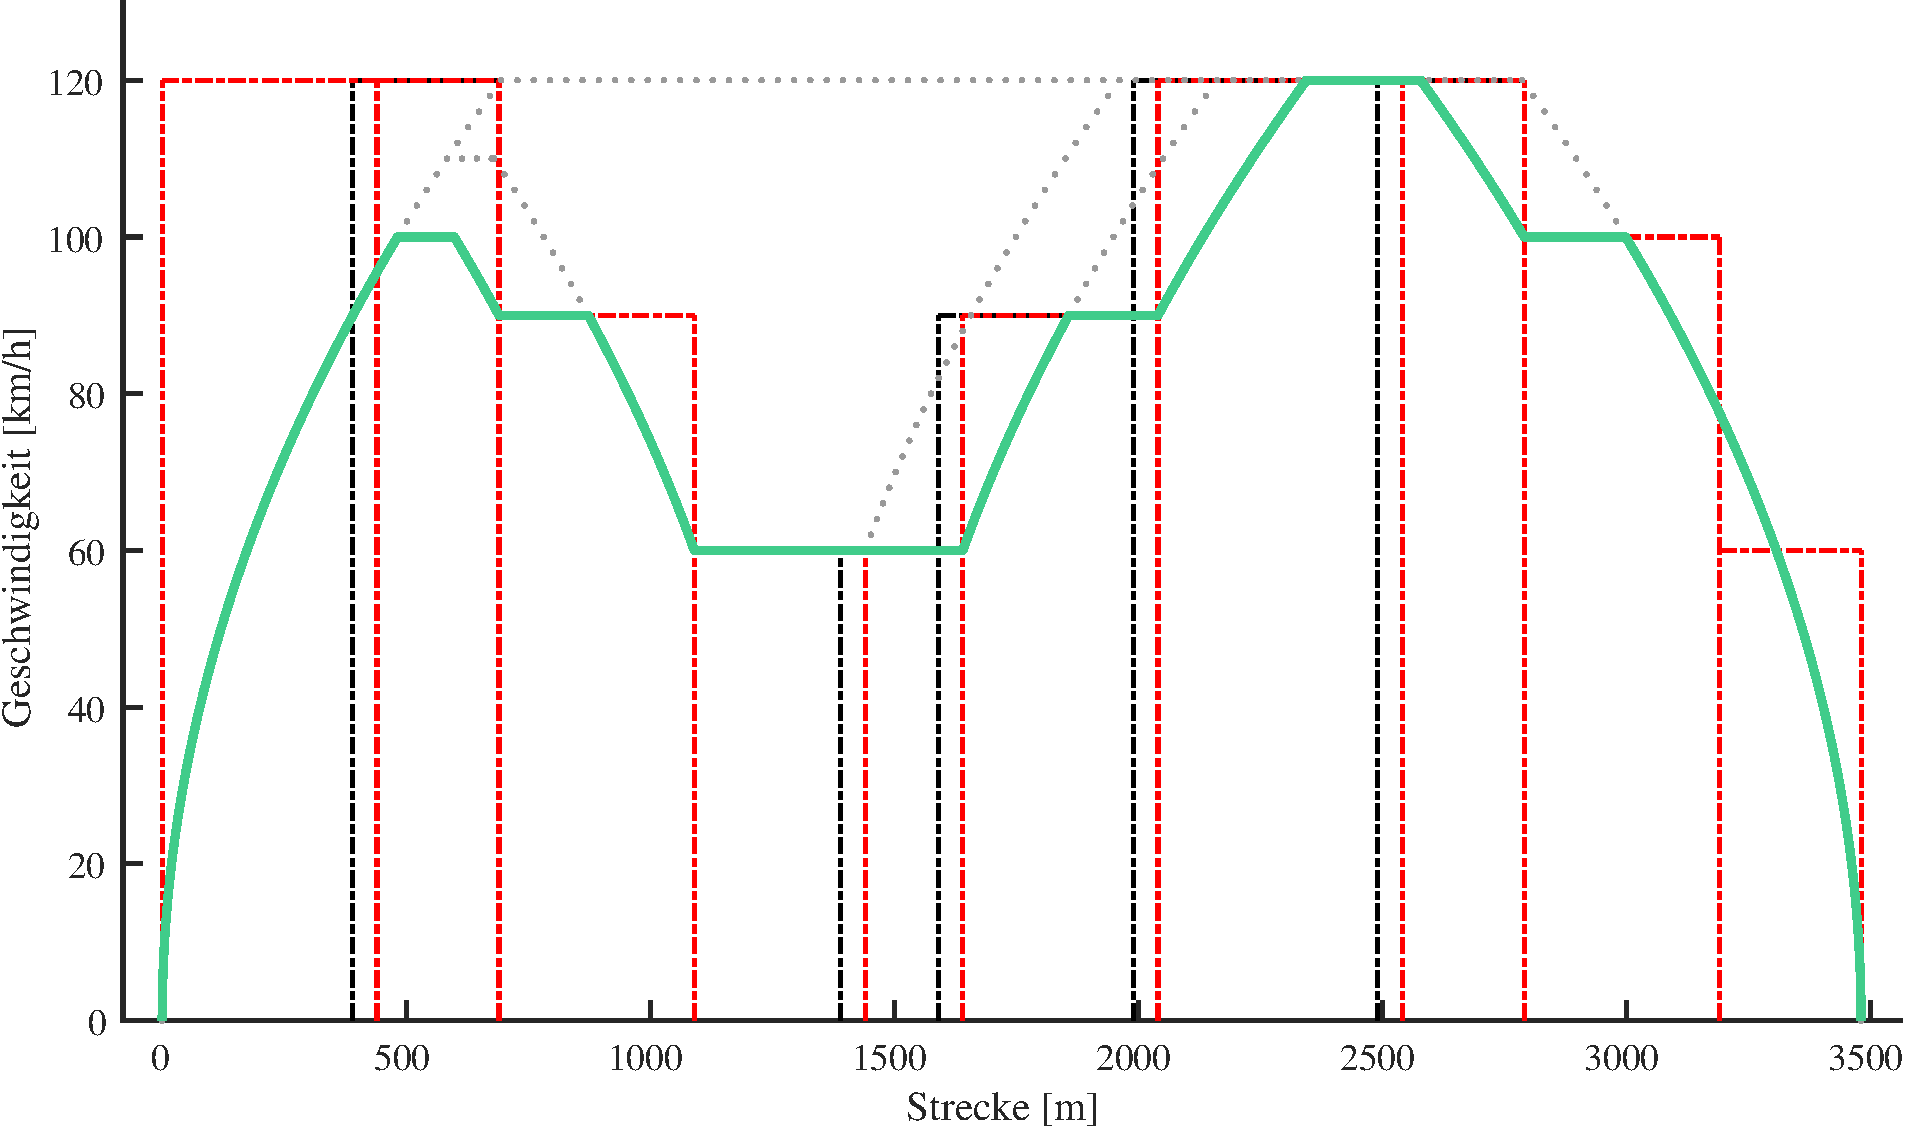
\includegraphics[width=\linewidth]{../matlab/it_4.pdf}
  \caption{Darstellung der Geschwindigkeit des Fahrzeugs über die Strecke}
\end{figure}
Lorem ipsum dolor sit amet, consetetur sadipscing elitr, sed diam nonumy eirmod tempor invidunt ut labore et dolore magna aliquyam erat, sed diam voluptua. At vero eos et accusam et justo duo dolores et ea rebum. Stet clita kasd gubergren, no sea takimata sanctus est Lorem ipsum dolor sit amet. Lorem ipsum dolor sit amet, consetetur sadipscing elitr, sed diam nonumy eirmod tempor invidunt ut labore et dolore magna aliquyam erat, sed diam voluptua. At vero eos et accusam et justo duo dolores et ea rebum. Stet clita kasd gubergren, no sea takimata sanctus est Lorem ipsum dolor sit amet.
\begin{figure}[H]
  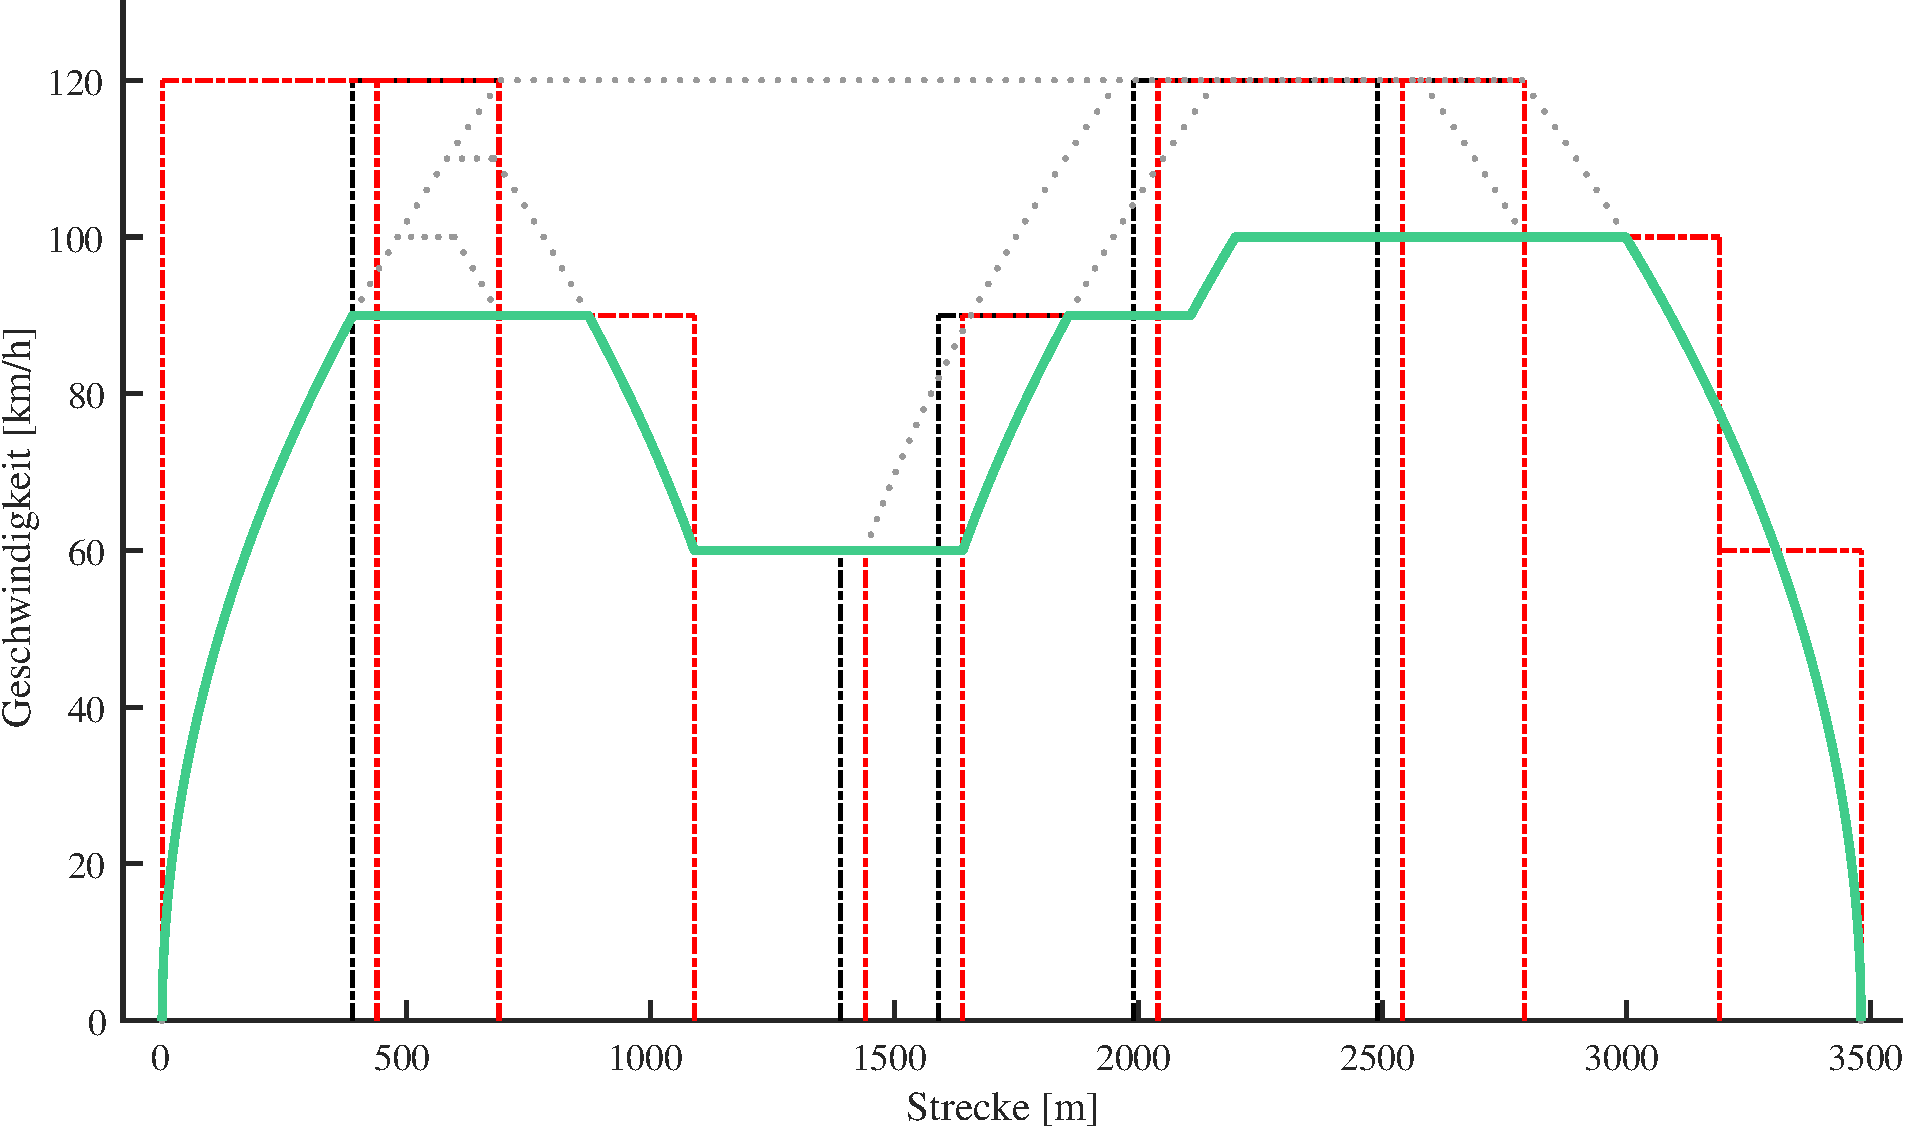
\includegraphics[width=\linewidth]{../matlab/it_5.pdf}
  \caption{Darstellung der Geschwindigkeit des Fahrzeugs über die Strecke}
\end{figure}
Lorem ipsum dolor sit amet, consetetur sadipscing elitr, sed diam nonumy eirmod tempor invidunt ut labore et dolore magna aliquyam erat, sed diam voluptua. At vero eos et accusam et justo duo dolores et ea rebum. Stet clita kasd gubergren, no sea takimata sanctus est Lorem ipsum dolor sit amet. Lorem ipsum dolor sit amet, consetetur sadipscing elitr, sed diam nonumy eirmod tempor invidunt ut labore et dolore magna aliquyam erat, sed diam voluptua. At vero eos et accusam et justo duo dolores et ea rebum. Stet clita kasd gubergren, no sea takimata sanctus est Lorem ipsum dolor sit amet.
\begin{figure}[H]
  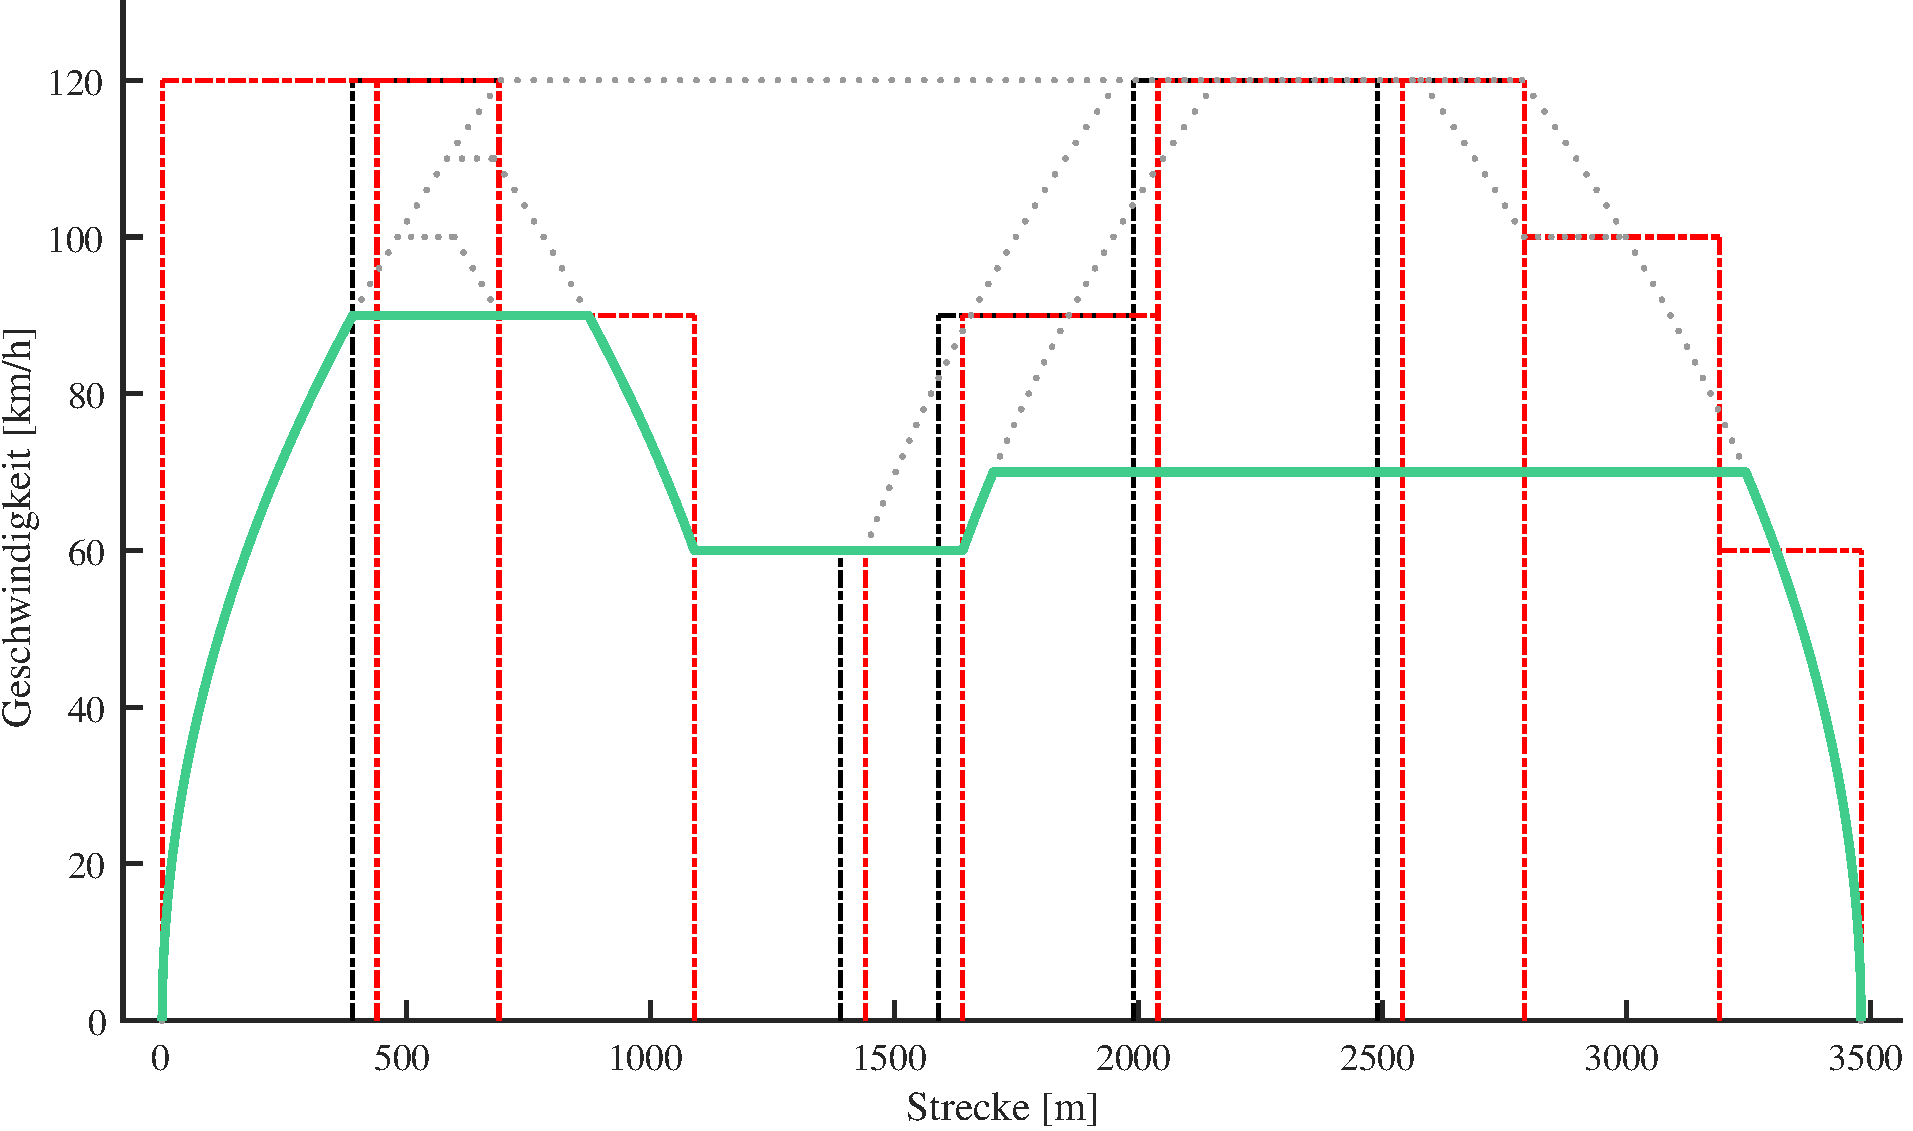
\includegraphics[width=\linewidth]{../matlab/it_6.pdf}
  \caption{Darstellung der Geschwindigkeit des Fahrzeugs über die Strecke}
\end{figure}
Lorem ipsum dolor sit amet, consetetur sadipscing elitr, sed diam nonumy eirmod tempor invidunt ut labore et dolore magna aliquyam erat, sed diam voluptua. At vero eos et accusam et justo duo dolores et ea rebum. Stet clita kasd gubergren, no sea takimata sanctus est Lorem ipsum dolor sit amet. Lorem ipsum dolor sit amet, consetetur sadipscing elitr, sed diam nonumy eirmod tempor invidunt ut labore et dolore magna aliquyam erat, sed diam voluptua. At vero eos et accusam et justo duo dolores et ea rebum. Stet clita kasd gubergren, no sea takimata sanctus est Lorem ipsum dolor sit amet.
\begin{figure}[H]
  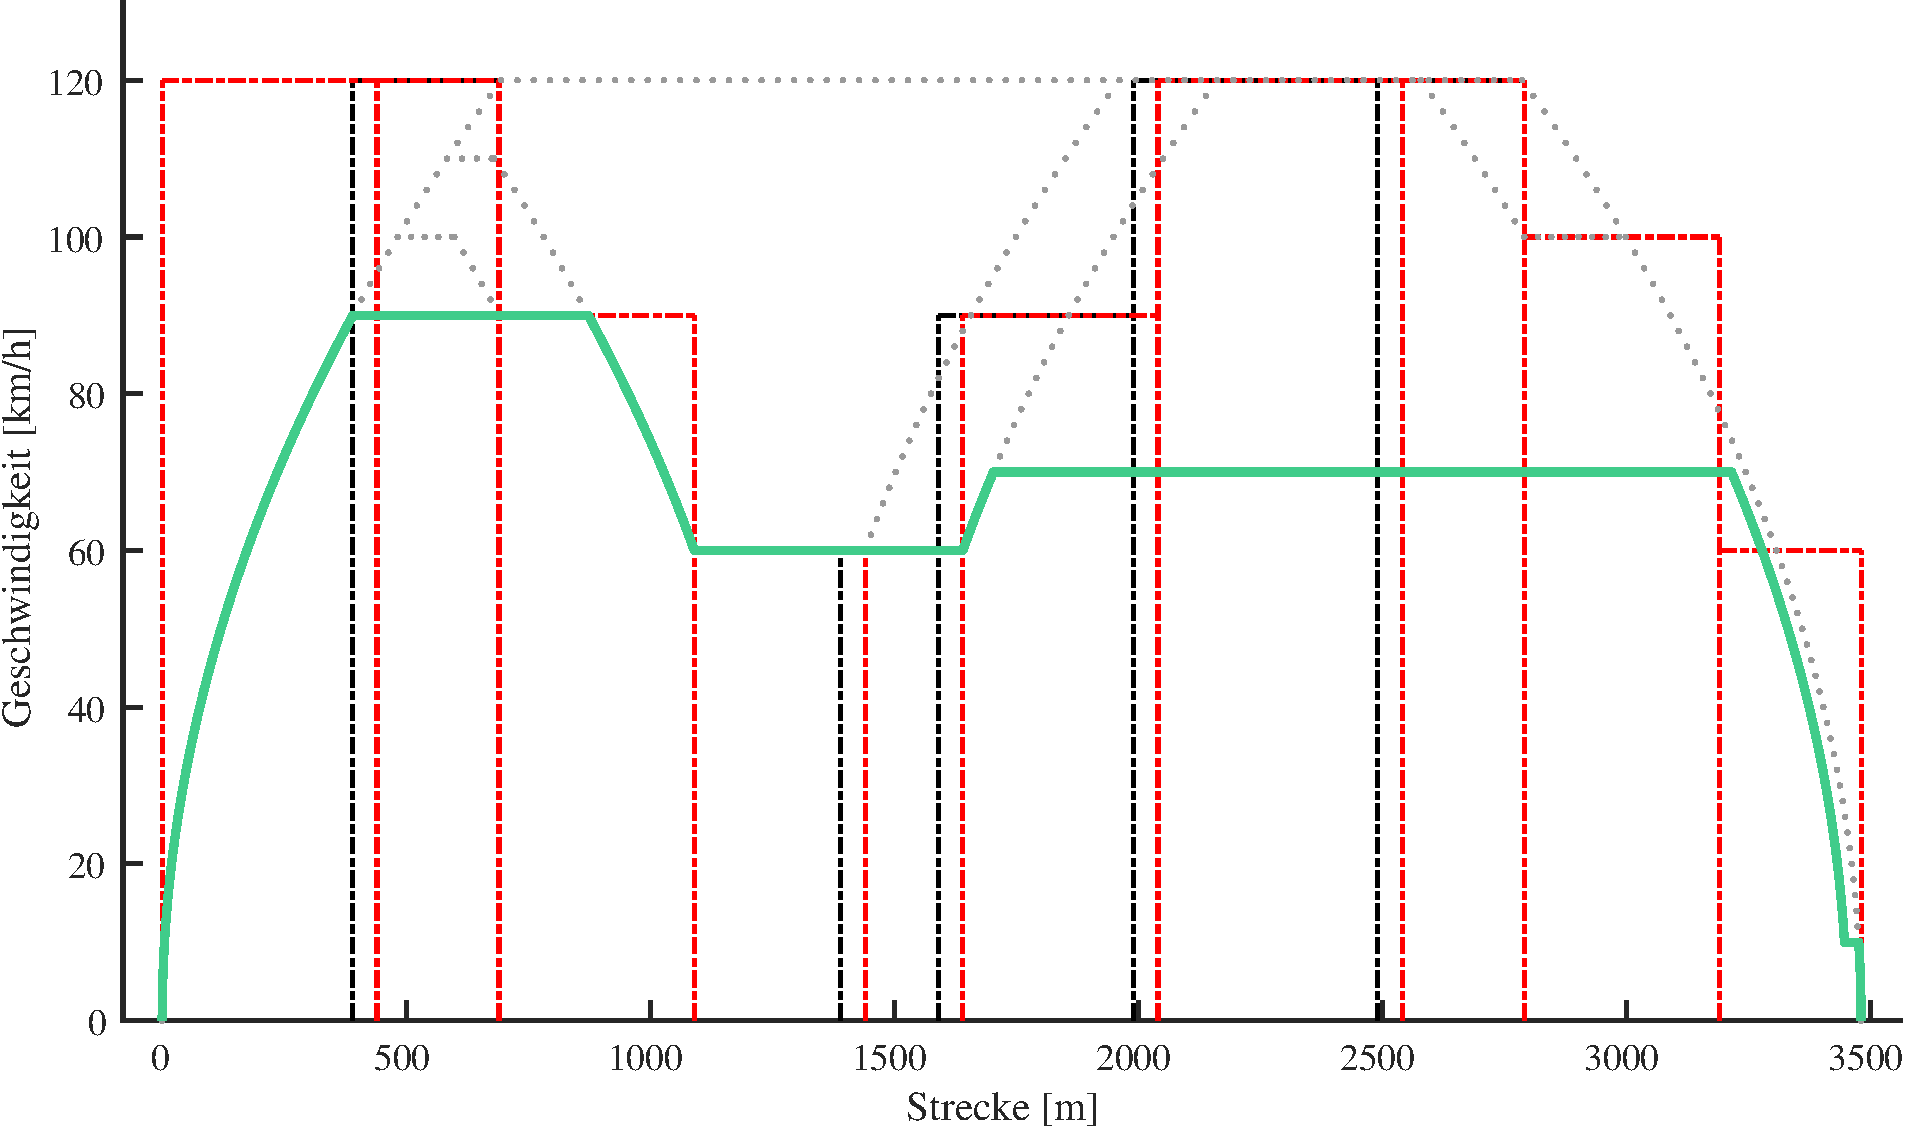
\includegraphics[width=\linewidth]{../matlab/it_7.pdf}
  \caption{Darstellung der Geschwindigkeit des Fahrzeugs über die Strecke}
\end{figure}



\subsection{speedFineTuning}

Es gilt:

\begin{equation}
\label{eq:t_ges}
t_{ges} = t_{1} + t_{2}
\end{equation}

\begin{equation}
\label{eq:s_ges}
s_{ges} = s_{1} + s_{2}
\end{equation}

\begin{equation}
\label{eq:s_v_t}
s = v \cdot t
\end{equation}
Durch das Einsetzen der Gleichung \eqref{eq:s_v_t} in die Gleichung \eqref{eq:s_ges} erhält man folgende Gleichung:
\begin{equation}
\label{eq:s_ges_2}
s_{ges} = v_{1} \cdot t_{1} + v_{2} \cdot t_{2}
\end{equation}
Durch das Umstellen der Gleichung \eqref{eq:t_ges} nach $t_{2}$ und dem Einsetzen in Gleichung \eqref{eq:s_ges_2} gilt für $t_{1}$:
\begin{equation}
t_{1} = \frac{s_{ges} - v_{2} \cdot t_{ges}}{v_{1} - v_{2}}
\end{equation}












